\icode[purple]{N14II-EXM-FI-L4-260625-001}
\nceeID[8]{2014新课标\Rmnum{2}}{22}
某实验小组探究弹簧的劲度系数\(k\)与其长度（圈数）的关系。实验装置如图（\(a\)）所示：一均匀长弹簧竖直悬挂，7个指针\(P_0\)、\(P_1\)、\(P_2\)、\(P_3\)、\(P_4\)、\(P_5\)、\(P_6\)分别固定在弹簧上距悬点0、10、20、30、40、50、60圈处：通过旁边竖直放置的刻度尺，可以读出指针的位置，\(P_0\)指向0刻度。设弹簧下端未挂重物时，各指针的位置记为\(x_0\)；挂有质量为\,\qty{0.100}{kg}的砝码时，各指针的位置记为\(x\)。测量结果及部分计算结果如表所示（\(n\)为弹簧的圈数，取重力加速度为\,\qty{9.80}{m/s^2}）。已知实验所用弹簧总圈数为60，整个弹簧的自由长度为\,\qty{11.88}{cm}。


	\begin{minipage}[c]{.2\textwidth}
		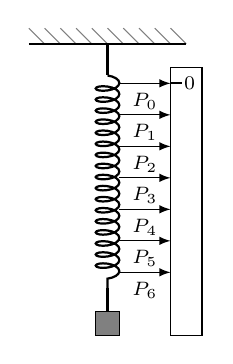
\begin{tikzpicture}
			\foreach \x in {-1,-.8,...,.8}
				\draw[gray] (\x,.2)--++(.2,-.2);
			\draw[thick] (-1,0)--(1,0) (0,0)--(0,-.4) (0,-3.1)--(0,-3.4) (.8,-.5)--(.95,-.5);
			\node at(.85,-.5)[right]{\scriptsize 0};
			\draw (.8,-.3) rectangle(1.2,-3.7);
			\draw[fill=gray] (-.15,-3.4) rectangle(.15,-3.7);
			\draw[thick,decoration={aspect=.4,segment length=4,amplitude=1.5mm,coil},decorate] (0,-.4)--(0,-3.1);
			\foreach \y/\n in {-.5/0,-.9/1,-1.3/2,-1.7/3,-2.1/4,-2.5/5,-2.9/6}
				\draw[-latex] (.15,\y)--node[below]{\scriptsize \(P_{\n}\)}(.8,\y);
		\end{tikzpicture}		
	\end{minipage}
	\begin{minipage}[c]{.65\textwidth}
		\begin{tabular}{|c|c|c|c|c|c|c|}
			\hline
			\diagbox{}{}&\(P_1\)&\(P_2\)&\(P_3\)&\(P_4\)&\(P_5\)&\(P_6\)\\
			\hline
			\(x_0\)(\qty{}{cm})&2.04&4.06&6.06&8.08&10.03&12.01\\
			\hline
			\(x\)(\qty{}{cm})&2.64&5.26&7.81&10.30&12.93&15.41\\
			\hline
			\(n\)&10&20&30&40&50&60\\
			\hline
			\(k\)(\qty{}{N/m})&163.3&\ding{192}&56.0&44.1&33.8&28.8\\
			\hline
			\(\frac{1}{k}\)(\qty{}{m/N})&0.0061&\ding{193}&0.0179&0.0227&0.0296&0.0347\\
			\hline
		\end{tabular}	
	\end{minipage}

	（1）将表中数据补充完整：\ding{192}\lunl{4em}，\ding{193}\lunl{4em}

	（2）以\(n\)为横坐标，\(\frac{1}{k}\)为纵坐标，在图（\(b\)）给出的坐标纸上画出\(\frac{1}{k} - n\)图象。
	\begin{figure}[htbp]
		\centering
		\begin{tikzpicture}[scale=1.2]
			\draw[help lines,color=gray!70,very thin,step=.1] (0,0)grid(6.2,4);
			\draw[help lines,color=black,thin,step=1] (0,0) grid(6,4);
			\draw[-latex,blue] (0,0)--(6.6,0)node[below]{\footnotesize \(n\)};
			\draw[-latex,blue] (0,0)--(0,4.6)node[right]{\footnotesize \(\frac{1}{k}\)/(\qty{}{m\cdot N^{-1}})};
			\foreach \x/\n in {0/0,1/10,2/20,3/30,4/40,5/50,6/60}
				\node at(\x,0)[below]{\footnotesize \(\n\)};
			\foreach \y/\n in {1/0.01,2/0.02,3/0.03,4/0.04}
				\node at(0,\y)[left]{\footnotesize \(\n\)};
		\end{tikzpicture}
	\end{figure}

	（3）图（\(b\)）中画出的直线可近似认为通过原点，若从实验中所用的弹簧截取圈数为\(n\)的一段弹簧，该弹簧的劲度系数\(k\)与其圈数\(n\)的关系的表达式为\(k =\) \lunl{4em}\,\qty{}{N/m}；该弹簧的劲度系数\(k\)与其自由长度\(l_0\)（单位为\,\qty{}{m}）的关系的表达式为\(k =\) \lunl{4em}\,\qty{}{N/m}